\vspace{-0.1cm}
\section{Retrying by Registration}
\label{sec:reg}
\vspace{-0.2cm}
When using a distance-based cost function for visual MPC it is necessary to update the belief of where the target object currently is, so that the agent can ``keep retrying" indefinitely until the task is accomplished. Prior work on visual MPC lacked this capability. To solve this issue we propose a method for registering the current image to both a start and goal image, where the designated pixels are known. In this way we can find the locations of the corresponding pixels in the \emph{current image} allowing us to compute the distances to the goal. Crucially, the registration method we propose is self-supervised using the same exact data for training the video prediction model and the registration model. This allows both the predictor and registration model to benefit from each episode of robot experience.

Before further detailing our learned registration system we discuss a two simple alternative approaches for obtaining a cost-function for video-prediction based control: One na\"{i}ve approach could be using the pixel-wise error between a \emph{goal image} and the \emph{predicted image}. However there are a number of issues with this approach: first when objects in the image are far from the position in the goal image (e.g., they do not overlap) there is no gradient signal with respect to changes in the actions. Second, due to the blurry predictions from a video prediction model, the pixel-wise difference between the predictions and the goal image can become meaningless. 

Another approach is to perform a registration between predicted video frames and the goal image and using the average length of the warping vectors as a cost function for ``closeness" to the goal image; however a major drawback of cost functions based on metrics computed on the complete image is that they naturally ``pay attention'' to large objects in the image (such as the arm) whereas small objects only contribute negligible amounts to the costs. As a result the planner only tries to match the positions of the big objects (the arm) ignoring smaller objects.

%The main contribution of this work is a method for computing the \emph{planning cost based on image-to-image registration}, which yields distances between a user-defined tracked object and its target location in the start or goal image. As a result, the cost is well-shaped, allowing for efficient optimization.

\begin{wrapfigure}{r}{.5\columnwidth}
\vspace{-0.25in}
\centering
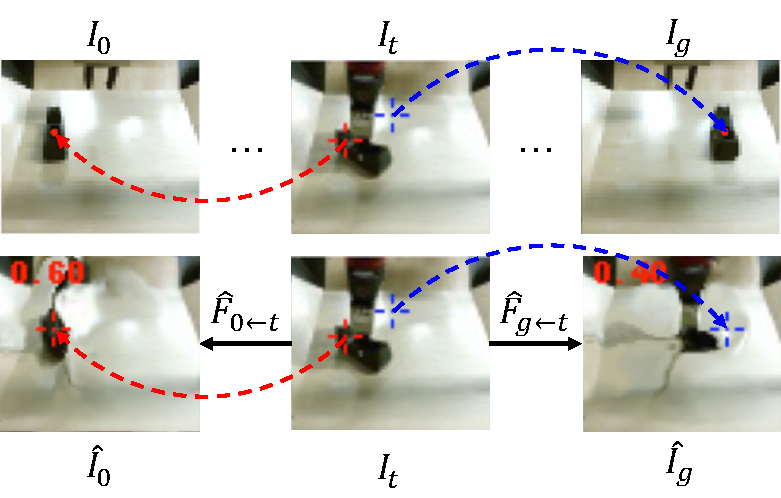
\includegraphics[width=0.5\columnwidth]{images/registration_singletime.pdf}
% \vspace{-0.1in}
\caption{\small{Closed loop control is achieved by registering the current image $I_t$ globally to the first frame $I_0$ and the goal image $I_g$. In this example registration to $I_0$ succeeds while registration to $I_g$ fails since the object in $I_g$ is too far away.}
\label{fig:reg_single}
\vspace{-0.2in}
}
\end{wrapfigure}

\subsection{Test time procedure}
 We will first describe the registration scheme at test time (see Figure~\ref{fig:registration_arch}(a)). We separately register the current image $I_t$ to the start image $I_0$ and to the goal image $I_g$ by passing it into registration network $R$, implemented as a fully-convolutional neural network. Additional details about the archiecture are given in section \ref{subsec:training}. The registration network produces a flow map $\hat{F}_{0 \leftarrow t} \in \mathbb{R}^{H \times W \times 2}$, a vector field with the same size as the image, that describes the relative motion for every pixel between two frames:
\begin{align}
    \hat{F}_{0 \leftarrow t} = R(I_t, I_0) &&
    \hat{F}_{g \leftarrow t} = R(I_t, I_g)
\end{align}

The flow map $\hat{F}_{0 \leftarrow t}$ can be used to warp the image of the current time step $t$ to the start image $I_0$, and $\hat{F}_{g \leftarrow t}$ can be used to warp from $I_t$ to $I_g$ (see Figure \ref{fig:reg_single} for an illustration):
\begin{align}
    \hat{I}_0 = \hat{F}_{0 \leftarrow t} \diamond  I_t &&
    \hat{I}_g = \hat{F}_{g \leftarrow t} \diamond  I_t 
\end{align}
where $\diamond$ denotes a bilinear interpolation operator that interpolates the pixel value bilinearly with respect to a location $(x,y)$ and its four neighbouring pixels in the image. In essence for a current image $\hat{F}_{0 \leftarrow t}$ puts $I_t$ in correspondence with $I_0$, and $\hat{F}_{g \leftarrow t}$ puts $I_t$ in correspondence with $I_g$. As one might expect warping works better for images that are closer to each other and sometimes fails when the entities in the image are too far apart. The motivation for registering both to $I_0$ and $I_g$ is to increase accuracy and robustness. In principle only one of either $I_0$ and $I_g$ are necessary. The goal-image can be provided by through a demonstration.

While the registration network is trained to perform a global registration between the images, we only evaluate it at the points $d_0$ and $d_g$ chosen by the user. This results in a cost function that ignores distractors. The flow map produced by the registration network is used to find the pixel locations corresponding to $d_0$ and $d_g$ in the current frame: 
\begin{align}
    \hat{d}_{0,t} = d_0 + \hat{F}_{0 \leftarrow t}(d_0) &&
    \hat{d}_{g,t} = d_g + \hat{F}_{g \leftarrow t}(d_g)
    \label{eqn:warped_pos}
\end{align}


\begin{figure}[t!]
    \centering
    \begin{subfigure}[b]{0.25\textwidth}
        \centering
        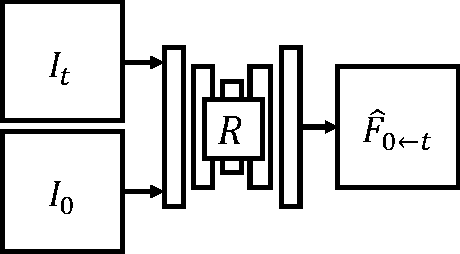
\includegraphics[width=\textwidth]{images/registration_test_start.pdf}\vspace{2.5mm}
        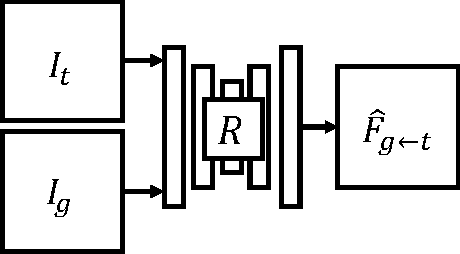
\includegraphics[width=\textwidth]{images/registration_test_goal.pdf}
        \caption{\small{Testing usage.}}
    \end{subfigure}
    \quad \quad
    \begin{subfigure}[b]{0.55\textwidth}
        \centering
        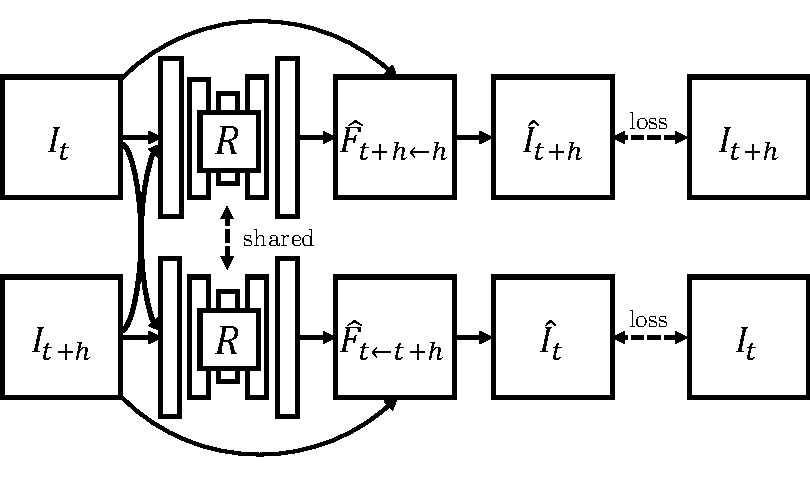
\includegraphics[width=\textwidth,trim={0 3mm 0 3mm},clip]{images/registration_train.pdf}
        \caption{\small{Training usage.}}
        \label{fig:discrete}
    \end{subfigure}
    \vspace{-1mm}
    \caption{\small{(a) At test time the registration network registers the current image $I_t$ to the start image $I_0$ (top) and goal image $I_g$ (bottom), inferring the flow-fields $\hat{F}_{0 \leftarrow t}$ and $\hat{F}_{g \leftarrow t}$. (b) The registration network is trained by warping images from randomly selected timesteps along a trajectory to each other.
    }}
    \label{fig:registration_arch}
\end{figure}

\begin{figure}
    \centering
    \vspace{-0.1in}
    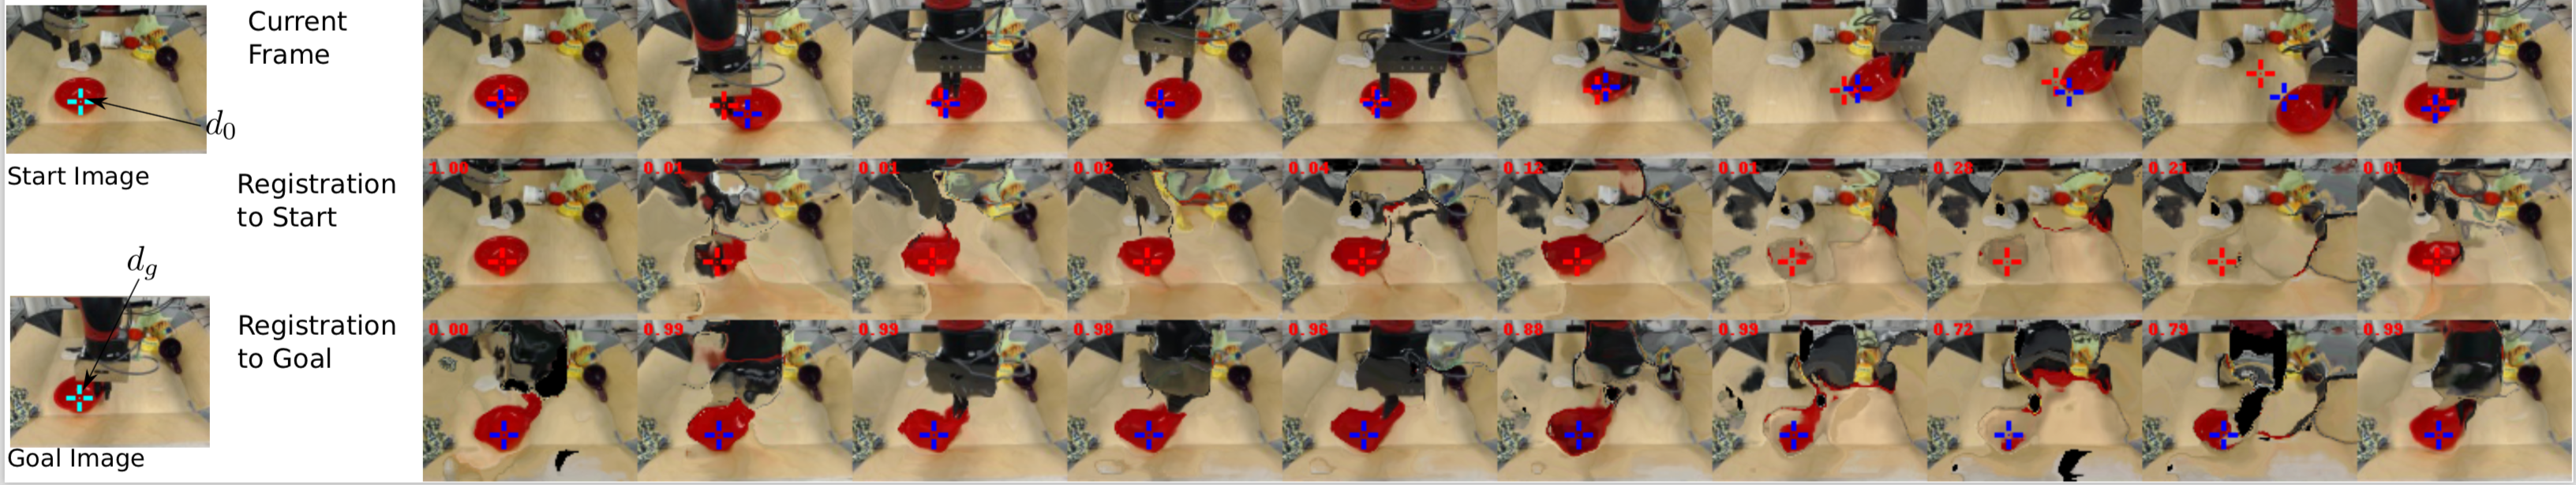
\includegraphics[width=1\textwidth]{images/reg_over_time.png}
    \caption{\small{Outputs of registration network. The first row shows the timesteps from left to right of a robot picking and moving a red bowl, the second row shows each image warped to the initial image via registration, and the third row shows the same for the goal image. A successful registration in this visualization would result in images that closely resemble the start- or goal image. In the first row, the locations where the designated pixel of the start image $d_0$ and the goal image $d_g$ are found are marked with red and blue crosses, respectively. It can be seen that the registration to the start image (red cross) is failing in the second to last time step, while the registration to the goal image (blue cross) succeeds for all time steps. The numbers in red, in the upper left corners indicate the trade off factors $\lambda$ between the views and are used as weighting factors for the planning cost. (Best viewed in PDF)}}
    \label{fig:tracking_overtime}
    \vspace{-0.2in}
\end{figure}

For simplicity we are showing only the case for one designated pixel. In practice, instead of a single flow vector $\hat{F}_{0 \leftarrow t}(d_0)$ and $\hat{F}_{g \leftarrow t}(d_g)$, we consider a neighborhood of flow-vectors around $d_0$ and $d_g$ and take the median in $x$ and $y$ directions making the registration more stable.
\autoref{fig:tracking_overtime} visualizes an example tracking result while the gripper is moving an object.

% On the left we show the start and goal image provided by the user at the beginning of the trajectory. The first row shows the video, with the estimated location of $d_0$ marked in red and the estimated location of $d_g$ marked in blue. In this example, registration succeeds with respect to the first image succeeds for the first 7 steps but fails after that (by successful registration we mean that the cross is on the object of interest). However registration with respect to the goal image, indicated by the blue cross succeeds for the last 3 steps. Thus, there is enough information at each time step to determine the planning cost.

%%SL.06.12: Something to keep in mind here: When describing a learned model, often a good recipe is to first explain the model itself (which is what you're doing here), and then explain how that model is trained. It's important to stick to good abstraction. If the model implementation (i.e., the neural net) is complicated, it can help to first explain it abstractly, then explain the objective, and only then explain how it is instantiated in a neural network. Perhaps this organization can be adopted in this section.



%SL.06.12: I think we need a separate paragraph that discusses two views... this paragraph seems to mix together two different things

%%SL.06.12: for top-level organization, we should have separate subsections for registration and for control. Maybe a reasonable top-level organization I might suggest is:
% 3 Preliminaries
% 4 Overview (summarize how the method works and say what the parts are, so the sections that follow don't come as a surprise)
% 5 Retrying with Registration
% 5.1 Self-Supervised Registration of Goal and Source Images <- this would have \paragraphs for algorithm, training/objective, and model
% 5.2 Deriving Planning Costs from Self-Supervised Registration <- can mention designated pixels here
% 6 Task Setup and Implementation <- all the stuff about how the task is set up, action space, etc
% of course, other organizations are possible, but maybe this gives a hint for how to get started



